\documentclass[11pt]{article}
\usepackage{geometry}                % See geometry.pdf to learn the layout options. There are lots.
\geometry{letterpaper}                   % ... or a4paper or a5paper or ... 
%\geometry{landscape}                % Activate for for rotated page geometry
%\usepackage[parfill]{parskip}    % Activate to begin paragraphs with an empty line rather than an indent
\usepackage{graphicx}
\usepackage{color}
\usepackage{amssymb}
\usepackage{epstopdf}
\usepackage{sectsty}
\usepackage[hyphens]{url}  %% be sure to specify the option 'hyphens'
\DeclareGraphicsRule{.tif}{png}{.png}{`convert #1 `dirname #1`/`basename #1 .tif`.png}

\title{Drake-Cullen-Part-1-Answers}
\author{Drake Cullen}
%\date{}                                           % Activate to display a given date or no date

\begin{document}
%\maketitle
%\section{}
%\subsection{}
\begin{minipage}{\linewidth}% to keep image and caption on one page
\centering

\includegraphics[keepaspectratio=true,scale=0.35]{CMU.png}
\end{minipage}
\section*{ \centering Task 1 Solutions}
\subsection*{ \centering By Drake Cullen} 

\vspace{5mm}
 
I declare that all material in this assessment task is my work except where there is clear acknowledgement or reference to the work of others. I further declare that I have complied and agreed to the CMU Academic Integrity Policy at the University website. http://www.coloradomesa.edu/student-services/documents
\begin{center}
\textbf{Author’s Name:} Drake Cullen 
\textbf{UID(700\#):} 700480375
\textbf{ Date:} 9/28/2021
\end{center} 

\section{Statement a)}
The statement is \textbf{True}. Start by finding the weight with the minimum value (smallest negative value). Add a constant factor large enough to make that value positive, and add that value to every other weight. Now, every weight is a positive value. We know that Dijkstras algorithm can be run on graphs with all positive values.

\newpage
\section{Statement b)}
The statement is \textbf{False}. Weights with a value of one cause a problem. Other positive integers will grow larger when squared, but one will keep the same value when squared; therefore, the weights won't increase proportionally. The statement would be true if every weight was multiplied by a constant such as 2. The manner in which the statement fails can be seen in the example below. 

\begin{center}
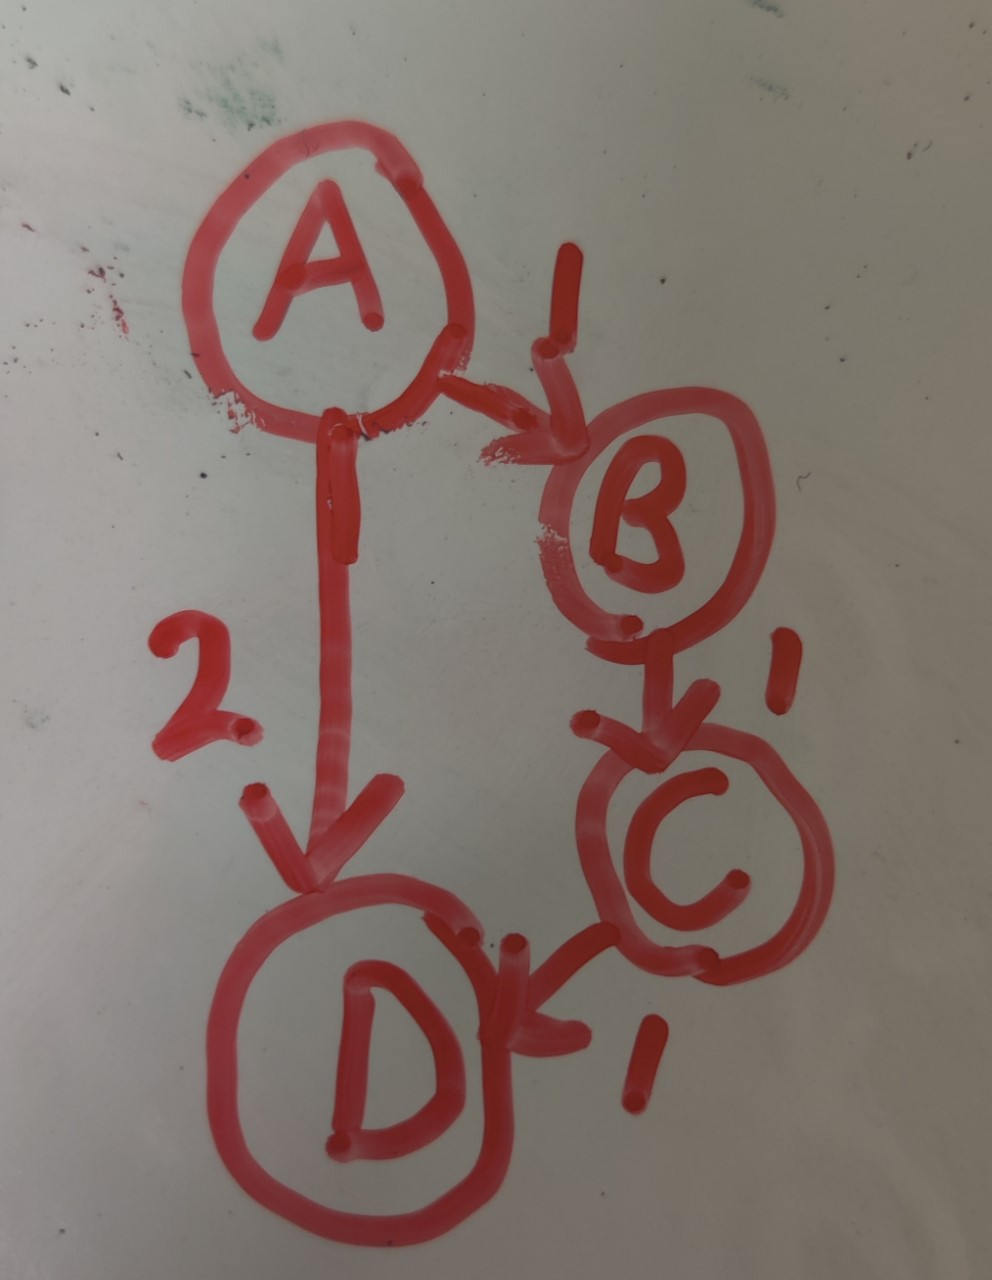
\includegraphics[keepaspectratio=true,scale=0.25]{graph2.jpg}
\end{center}
Let us assume that you are looking for the shortest path from A to D using the graph above. There are two different paths that you can take to get from A to D.

\begin{center}
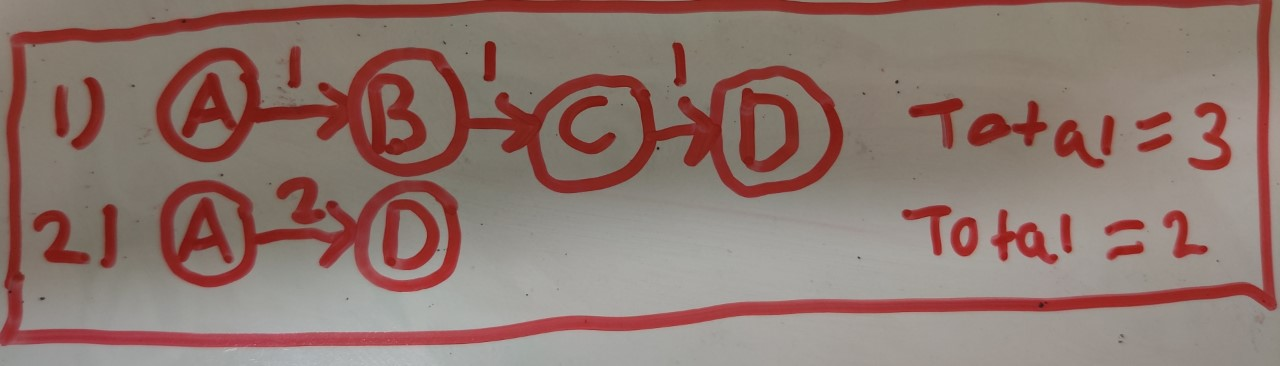
\includegraphics[keepaspectratio=true,scale=0.25]{original_paths2.jpg}
\end{center}
By taking the path from A to B to C to D (call this path1), the combined weight is 3. If you choose to take the path2 from A to D, the combined weight is 2. Therefore, path2 is shorter than path1.

\begin{center}
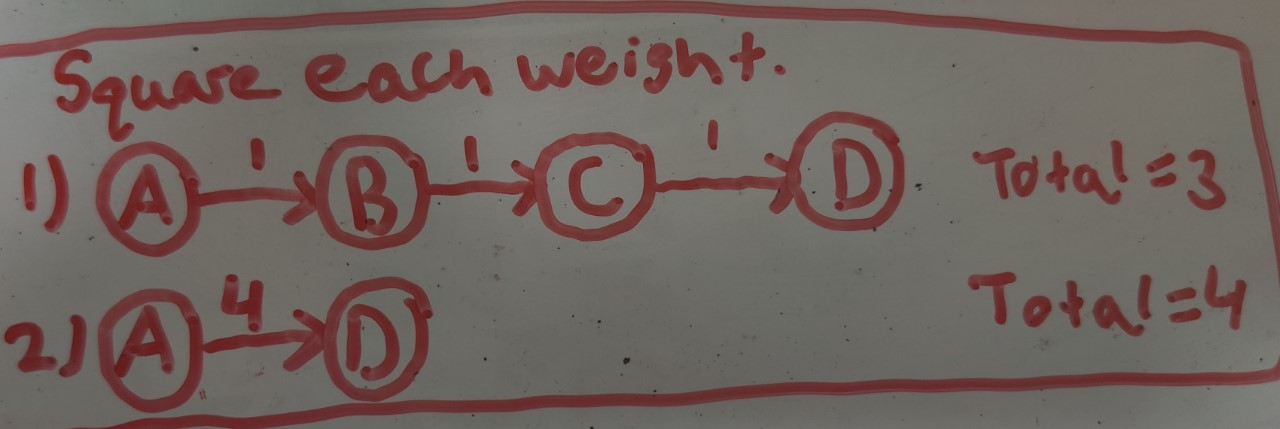
\includegraphics[keepaspectratio=true,scale=0.25]{updated_paths2.jpg}
\end{center}
After squaring every edge, the updated paths can be seen in the image above. Path1 is now shorter than path2. We know that path2 should be shorter than path1, so by squaring every edge, the shortest path is now innacurate; therefore, this statement is false.

\end{document}  